%%%%%%%%%%%%%%%%%%%%%%%%%%%%%%%%%%%%%%%%%
% a0poster Portrait Poster
% LaTeX Template
% Version 1.0 (22/06/13)
%
% The a0poster class was created by:
% Gerlinde Kettl and Matthias Weiser (tex@kettl.de)
% 
% This template has been downloaded from:
% http://www.LaTeXTemplates.com
%
% License:
% CC BY-NC-SA 3.0 (http://creativecommons.org/licenses/by-nc-sa/3.0/)
%
%%%%%%%%%%%%%%%%%%%%%%%%%%%%%%%%%%%%%%%%%

%----------------------------------------------------------------------------------------
%	PACKAGES AND OTHER DOCUMENT CONFIGURATIONS
%----------------------------------------------------------------------------------------

\documentclass[a0,portrait]{a0poster}

\usepackage{multicol} % This is so we can have multiple columns of text side-by-side
\columnsep=100pt % This is the amount of white space between the columns in the poster
\columnseprule=3pt % This is the thickness of the black line between the columns in the poster

\usepackage[svgnames]{xcolor} % Specify colors by their 'svgnames', for a full list of all colors available see here: http://www.latextemplates.com/svgnames-colors

\usepackage{times} % Use the times font
%\usepackage{palatino} % Uncomment to use the Palatino font

\usepackage{graphicx} % Required for including images
\graphicspath{{figures/}} % Location of the graphics files
\usepackage{booktabs} % Top and bottom rules for table
\usepackage[font=small,labelfont=bf]{caption} % Required for specifying captions to tables and figures
\usepackage{amsfonts, amsmath, amsthm, amssymb} % For math fonts, symbols and environments
\usepackage{wrapfig} % Allows wrapping text around tables and figures

\begin{document}

%----------------------------------------------------------------------------------------
%	POSTER HEADER 
%----------------------------------------------------------------------------------------

% The header is divided into two boxes:
% The first is 75% wide and houses the title, subtitle, names, university/organization and contact information
% The second is 25% wide and houses a logo for your university/organization or a photo of you
% The widths of these boxes can be easily edited to accommodate your content as you see fit

\begin{minipage}[b]{0.92\linewidth}
\veryHuge \color{NavyBlue} \textbf{Estimating Energy Cost of continuous Context-sensing with Smartphone-embedded and neighborhood sensors} \color{Black}\\ % Title
\Huge\textit{ITRA Project: HumanSense - Development and deployment of mobile based systems for preliminary data collection to guide future directions of the project
 }\\[0.3cm] % Subtitle
\huge \textbf{Narendra Kumar Shukla \& Debopam Acharya}\\[0.3cm] % Author(s)
\huge Department of Computer Science and Engineering, Shiv Nadar University\\[0.3cm] % University/organization
\Large \texttt{narendra.shukla@ieee.org, debopam.acharya@snu.edu.in}\\
\end{minipage}
%
\begin{minipage}[b]{0.10\linewidth}

\includegraphics[width=8cm]{snulogo.png}\\
\end{minipage}
\vspace{0.5cm} % A bit of extra whitespace between the header and poster content

%----------------------------------------------------------------------------------------

\begin{multicols}{2} % This is how many columns your poster will be broken into, a portrait poster is generally split into 2 columns

%----------------------------------------------------------------------------------------
%	ABSTRACT
%----------------------------------------------------------------------------------------

%\color{Navy} % Navy color for the abstract
%
%\begin{abstract}
%Energy cost optimization while using off-the-shelf  Smartphones for continuous and accurate context sensing \\
%Context in our current work implies localized environmental data like temperature, humidity, atmospheric pressure, air/noise/water pollution parameters\\
%Increase in number of on-board sensors sensing continuously leads to complications due to inter-sensor-interactions and/or their usage scenarios. \\
%Contemporary smartphones with embedded sensors interacting with neighborhood sensors on Sensordrone platform using Bluetooth 2.1 \\
%Developed on-line-on-device profiler with offline measurements to build device specific power models for Samsung Galaxy S4 and Google Nexus 5\\
%Used profiler application for energy aware preliminary environment data collection and energy monitoring\\
%Online on-device profiler is most convenient for energy measurement; however, it introduces bias and becomes the top energy hog itself.

%In this work we have focused on energy-efficient continuous and collaborative context sensing with embedded sensors of Smartphone as well as neighborhood sensors that are pushing the data over radio to the Smartphone. Specifically, we propose to measure and estimate energy cost of continuous context sensing using embedded sensors of Smartphone and other neighborhood sensors. We are using Sensorcon's Sensordrone platform that has a collection of sensors for context-sensing and it communicates with the Smartphone using Bluetooth Low Energy Radio channel. We have conducted a series of experiments using on-device profilers, followed by customized set-up for offline power consumption measurement and power model generation. Our results indicate that an online on-device profiler is most convenient for energy measurement in continuous context data collection application using a crowd sourcing but it introduces bias and becomes the top energy hog itself. We have proposed a power model for Samsung Galaxy S4 Smartphone which is used to develop an energy efficient on-line-on-device profiler.
%Problem and generic solution.

%\end{abstract}


%----------------------------------------------------------------------------------------
%	OBJECTIVES
%----------------------------------------------------------------------------------------

%color{DarkSlateGray} % DarkSlateGray color for the rest of the content
%
\color{SaddleBrown}
\section*{Objectives}
%
\color{DarkSlateGray}
\begin{enumerate}
\item Develop suitable mobile applications pertaining to different aspects of the proposal
\item Use the developed applications for energy aware preliminary data collection in real environments
\item Create mobile based system, incorporating both the applications and sensing systems for broader applicability in healthcare and energy domain

%\item Lorem ipsum dolor sit amet, consectetur.
%\item Nullam at mi nisl. Vestibulum est purus, ultricies cursus volutpat sit amet, vestibulum eu.
%\item Praesent tortor libero, vulputate quis elementum a, iaculis.
%\item Phasellus a quam mauris, non varius mauris. Fusce tristique, enim tempor varius porta, elit purus commodo velit, pretium mattis ligula nisl nec ante.
%\item Ut adipiscing accumsan sapien, sit amet pretium.
%\item Estibulum est purus, ultricies cursus volutpat
%\item Nullam at mi nisl. Vestibulum est purus, ultricies cursus volutpat sit amet, vestibulum eu.
%\item Praesent tortor libero, vulputate quis elementum a, iaculis.
\end{enumerate}

%----------------------------------------------------------------------------------------
%	INTRODUCTION
%----------------------------------------------------------------------------------------

\color{SaddleBrown} % SaddleBrown color for the introduction

\section*{Energy aware preliminary data collection}
\color{DarkSlateGray} % DarkSlateGray color for the rest of the content
\begin{enumerate}
\item Context in our current work implies localized environmental data like temperature, humidity, atmospheric pressure, air/noise/water pollution parameters
\item Increase in number of on-board sensors sensing continuously leads to complications due to inter-sensor-interactions and/or their usage scenarios
\item Used Contemporary smartphones with embedded sensors interacting with neighborhood sensors on Sensordrone platform using Bluetooth 2.1
\item Developed on-line-on-device profiler with offline measurements to build device specific power models for Samsung Galaxy S4 and Google Nexus 5

\end{enumerate}
%\begin{center}\vspace{1cm}
%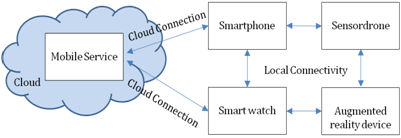
\includegraphics[width=0.6\linewidth]{setup}
%\captionof{figure}{\color{Green} Generic Crowsourcing Mobile System}
%\end{center}\vspace{1cm}

%----------------------------------------------------------------------------------------
%	EXPERIMENTAL SETUP
%----------------------------------------------------------------------------------------
\color{SaddleBrown}
\section*{Experimental Setup}

%\begin{columns} % Subdivide the first main column
%\begin{column}{.3\textwidth} % The first subdivided column within the first main column
%\centering
%\begin{figure}
%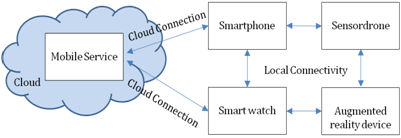
\includegraphics[width=0.9\linewidth, height=6cm]{setup}
%\caption{\small Sensing System}
%\end{figure}
%\end{column}
%
%\begin{column}{.3\textwidth} % The first subdivided column within the first main column
%\centering
%\begin{figure}
%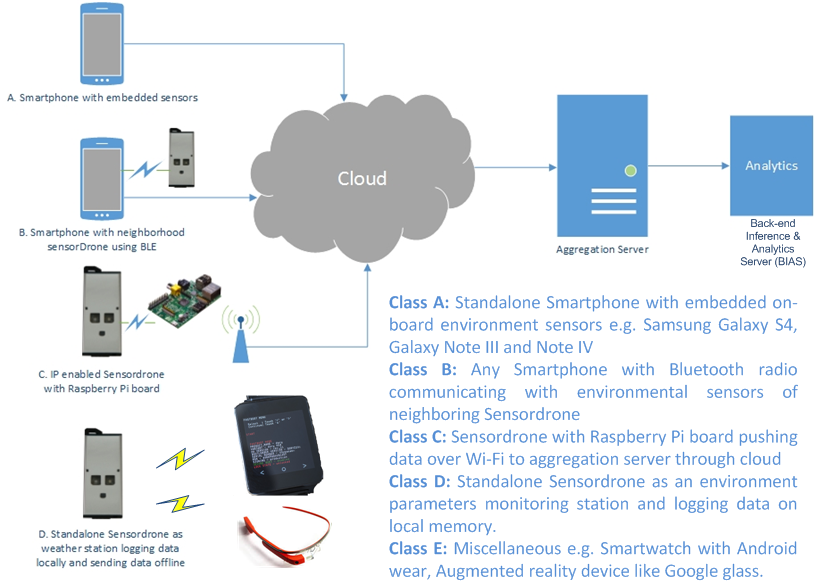
\includegraphics[width=0.9\linewidth, height=6cm]{Archi}
%\caption{\small Schematic for experimental study}
%\end{figure}
%\end{column}
%
%\end{columns} % End of the subdivision



\begin{center}
%\vspace{1cm}
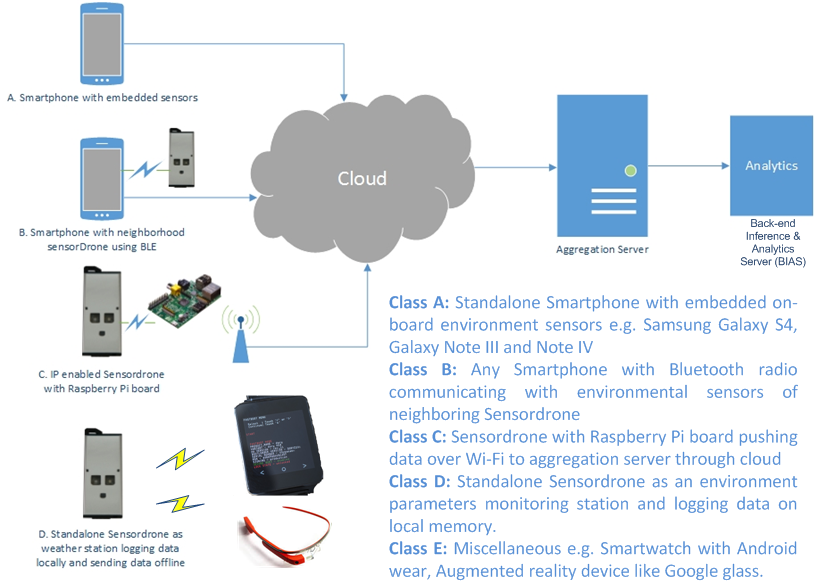
\includegraphics[width=0.8\linewidth]{Archi}
\captionof{figure}{\color{Green} Schematic of our system for experimental study}
\end{center}\vspace{1cm}

%------------------------------------------------
\color{SaddleBrown} % DarkSlateGray color for the rest of the content
\subsection*{Building Power Model of Online Profiler}
\color{DarkSlateGray}
Extended PowerBooter model:
%\begin{equation}
\begin{multline}
%\begin{align}
(\beta_{uh} \times freq_h + \beta_{ul} \times freq_l) \times util + \beta_{CPU} \times CPU_{on}
+ \beta_{br} \times AMOLED_{brightness} \\ 
+ \beta_{Gon} \times GPS_{\_on} + \beta_{Gsl} \times GPS_{\_sl}
+ \beta_{WiFi\_l} \times WiFi_l + \beta_{WiFi\_h} \times WiFi_h\\ 
+ \beta_{3G\_idle} \times 3G_{idle} 
+ \beta_{3G\_FACH} \times 3G_{FACH}
+ \beta_{3G\_DCH} \times 3G_{DCH} \\
+ \beta_{4G\_RRC\_idle} \times 4G_{RRC\_idle}
+ \beta_{4G\_RRC\_connected} \times 4G_{RRC\_connected} \\
+ \beta_{sensor} \times Sensor_{ON}
+ \beta_{Bluetooth\_2.1} \times Bluetooth_{2.1}
\label{eqn:Proposed Power Model for Samsung Galaxy S4}
%\end{\align}
\end{multline}
%\end{equation}
%β
where $\beta$ is  power coefficient and $util, CPU_{ON}....  etc.$ are utilization factor for a particular component (system variables). We use customized set-up to measure power consumption traces represented by P matrix. After collecting power traces in controlled environment, we use multi-variable regression to minimize Sum of Square errors for $\beta$ vector.\\
\begin{equation}
%$P= \beta U+c$\\
P= \beta U+c
\end{equation}
where $P$ vector is $n \times 1$ measured power values, $\beta$ vector is $1 \times m$ power coefficients to be estimated and U is  $m \times n$ matrix; where $U_{ij}$ represents system variable $ i$ in $j_{th}$ state. Constant $c$ is minimum power consumed on the device.

\begin{equation}
%$P= \beta U+c$\\
18.8 + 70.1 \times x - 22.4 \times x^2 +  4.4 \times x^3 - 0.4 \times x^4 + 0.01 \times x^5
\end{equation}

\begin{equation}
%$P= \beta U+c$\\

\end{equation}


\begin{center}\vspace{1cm}
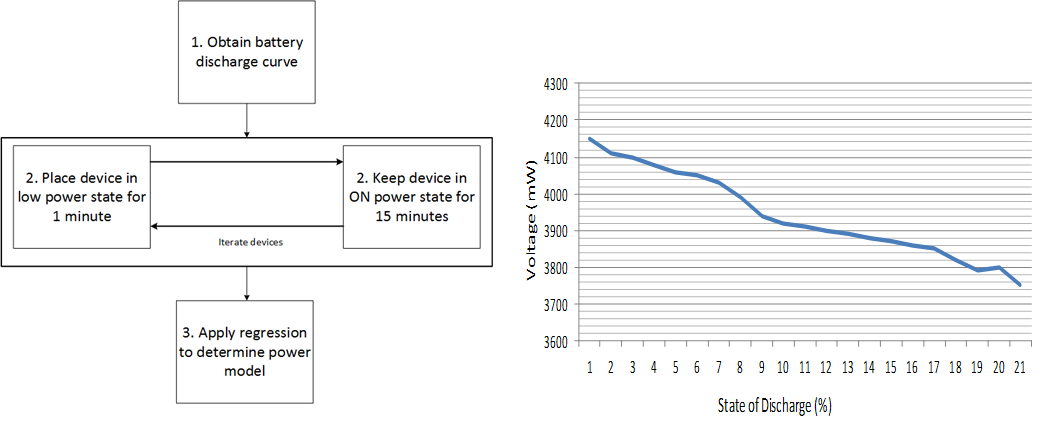
\includegraphics[width=0.8\linewidth]{PowerBooter}
\captionof{figure}{\color{Green} Key Phases of the proposed power Model and discharge curve for S4}
\end{center}\vspace{1cm}
\color{SaddleBrown}
\subsection*{Custom Setup for Power Measurement and Trace Analysis for S4 and Nexus5}
\color{DarkSlateGray}
\begin{center}\vspace{1cm}
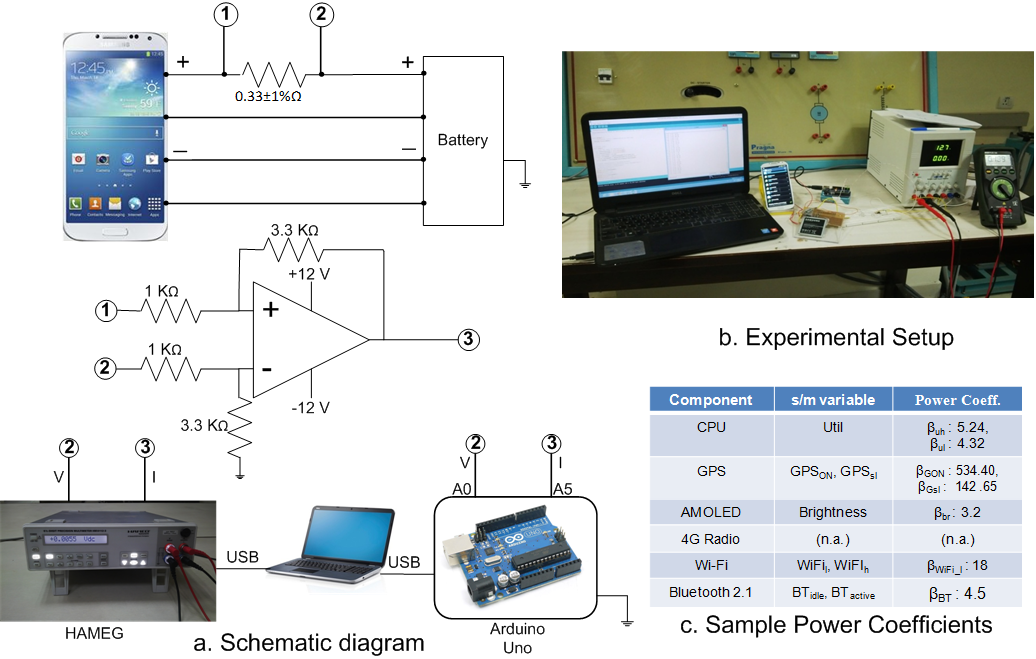
\includegraphics[width=1.0\linewidth]{CustomSetUpNew2}
\captionof{figure}{\color{Green} Custom setup for online power consumption estimation}
\end{center}\vspace{1cm}
HAMEG HM 8112-3 precision Multi-meter and Arduino Uno for measuring component level power-consumption. Our proposed model for S4 does not consider presence of sensor hub along with onboard power management module to reduce wake-up time of Master CPU by Android apps.%  as shown in Figure (4)
%
%\begin{center}\vspace{1cm}
%\includegraphics[width=0.4\linewidth]{sensorhub}
%\captionof{figure}{\color{Green} Sensorhub for energy saving in Samsung Galaxy S4}
%\end{center}\vspace{1cm}

%----------------------------------------------------------------------------------------
%	RESULTS 
%----------------------------------------------------------------------------------------
\color{SaddleBrown}
\section*{Results}
\color{DarkSlateGray}

\begin{center}\vspace{0.5cm}
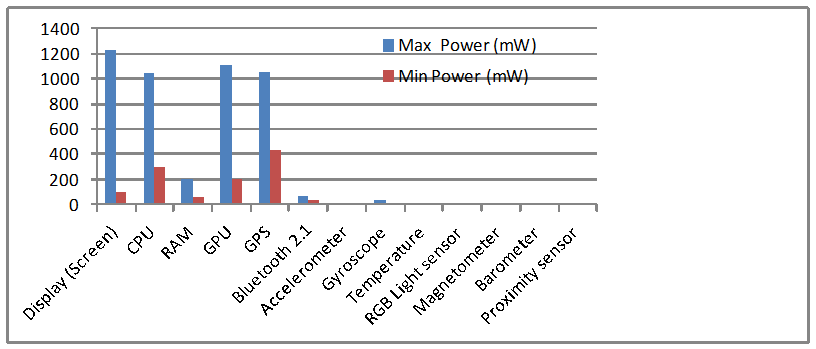
\includegraphics[width=0.9\linewidth]{Result}
\captionof{figure}{\color{Green} Average Component-wise Energy Consumption for Samsung Galaxy S4}
\end{center}\vspace{0.5cm}

\begin{center}\vspace{0.5cm}
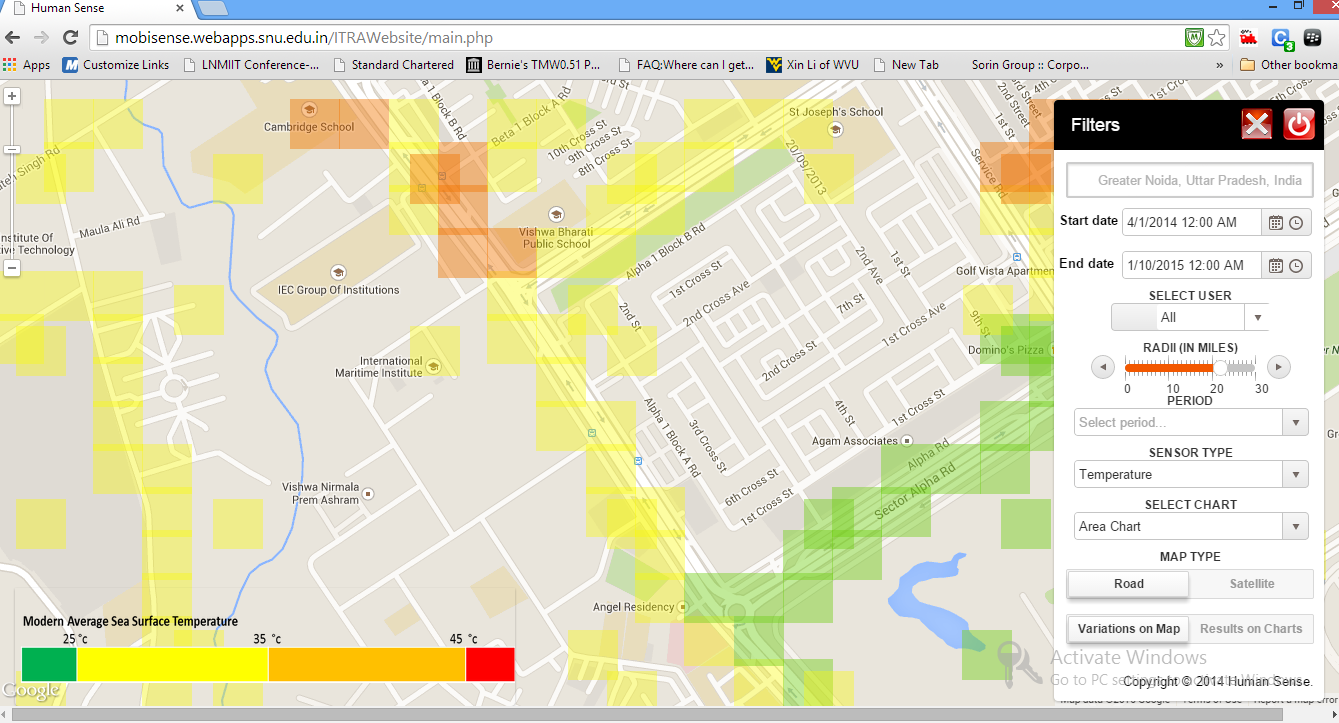
\includegraphics[width=0.8\linewidth]{Server}
\captionof{figure}{\color{Green} BIAS map of the Collected Data}
\end{center}\vspace{0.5cm}


%----------------------------------------------------------------------------------------
%	CONCLUSIONS AND FUTURE WORK
%----------------------------------------------------------------------------------------

\color{SaddleBrown} % SaddleBrown color for the conclusions to make them stand out

\section*{Conclusions and Future Work}
\color{DarkSlateGray} % Set the color back to DarkSlateGray for the rest of the content
\begin{itemize}
\item Online on device profiling is most convenient but it introduces bias and profiler itself becomes energy hog.
\item Offline setup or using power monitor like Monsoon is accurate but less desirable for continuous context sensing
\item Presence of sensor hub makes power modeling for latest Smartphones less accurate. 
\end{itemize}

\color{DarkSlateGray} % Set the color back to DarkSlateGray for the rest of the content

%----------------------------------------------------------------------------------------
%	FORTHCOMING RESEARCH
%----------------------------------------------------------------------------------------
%\color{SaddleBrown}
%\section*{Forthcoming Research}
%\color{DarkSlateGray}
%\begin{itemize}
%\item Correcting power model of S4 to develop fine grained profiler based on Amobisense
%\item Energy saving in making 802.11 also part of Sensor Hub
%\item How much LE is Bluetooth LE?
%\item Using CoAP for accessing data from Class C context monitoring device
%\end{itemize}

%\color{SaddleBrown}
% %----------------------------------------------------------------------------------------
%%	REFERENCES
%%----------------------------------------------------------------------------------------
%\nocite{*} % Print all references regardless of whether they were cited in the poster or not
%\bibliographystyle{plain} % Plain referencing style
%\bibliography{sample} % Use the example bibliography file sample.bib

%----------------------------------------------------------------------------------------
%	ACKNOWLEDGEMENTS
%----------------------------------------------------------------------------------------
\color{SaddleBrown}
\section*{Acknowledgements}
\color{DarkSlateGray}
%\begin{itemize}
ITRA research grant HumanSense: Towards context aware sensing, inference and actuation for applications in Energy and Healthcare, under the Department of Electronics and Information Technology, Government of India.
%\item Team: Debopam Acharya (Associate Professor), Prasad Pathak (Assistant Professor), Rahul Majethia (PhD Student)
%Narendra Shukla (PhD Student), Varun Mishra, Meghna Joshi, Arihant Lunkar, Bakul Budhiraja, Deepika Mann (Project Assistants)
%\end{itemize}
%----------------------------------------------------------------------------------------
%	YEAR ONE TEAM SNU
%----------------------------------------------------------------------------------------
\color{SaddleBrown}
\section*{Year one Team SNU}
\color{DarkSlateGray}
\begin{itemize}
\item Debopam Acharya (Associate Professor), Prasad Pathak (Assistant Professor), Rahul Majethia (PhD Student)
Narendra Shukla (PhD Student), Varun Mishra, Meghna Joshi, Arihant Lunkar, Bakul Budhiraja, Deepika Mann (Project Assistants)
\end{itemize}

%----------------------------------------------------------------------------------------
\end{multicols}
\end{document}